% ------------------------------------------------------------------------
% Poster: Modelo de Poster para eventos de Lic. Inform.
%
% Template por Francisco Reinaldo
%		(https://orcid.org/0000-0001-6161-6755)
%		(http://lattes.cnpq.br/7401534350061823)
% ------------------------------------------------------------------------
% Agradecimentos a Overleaf pela oportunidade
% ------------------------------------------------------------------------

\def\footer#1{\def\insertfooter{#1}}
\documentclass[final]{beamer}

\usepackage[scale=1.150]{beamerposter}
\usetheme{MUWposter}

%\logo{\pgfputat{\pgfxy(-13,108.5)}{\pgfbox[center,base]{
\includegraphics[width=18cm]{logo_UTFPR.jpg}}}}

\usepackage{multicol}
\usepackage{array}
%The following two are column definitions for the aknowledgements section
\newcolumntype{L}{>{\arraybackslash}m{22cm}}
\newcolumntype{S}{>{\arraybackslash}m{5cm}}
\usepackage{pgf}
\usepackage{mathtools}
\usepackage{amsmath, amsthm, amssymb, amsfonts}
\usepackage{exscale}
\usepackage{xcolor}
\usepackage{ushort}
\usepackage{setspace}
\usepackage[square,numbers]{natbib}
\usepackage{url}
\bibliographystyle{abbrvnat}
\renewcommand{\vec}[1]{\ushort{#1}}
\renewcommand{\vec}[1]{\mathbf{#1}}
\definecolor{greenMUW}{RGB}{60,191,174}
\definecolor{blueMUW}{RGB}{17,29,79}
\definecolor{skinMUW}{RGB}{254,228,217}
\definecolor{hellblauMUW}{RGB}{95,180,229}
\usepackage{xcolor}
\usepackage{graphicx}
%-----------------------------------------------
%  START Set the colors
%  Uncomment to apply colors you want to use.
%-----------------------------------------------
\colorlet{themecolor}{greenMUW}
\usebackgroundtemplate{\includegraphics[width=90cm,height=120cm]{MUW_green}}


%-----------------------------------------------
%  START Set the width of the columns
%-----------------------------------------------
\setlength{\paperwidth}{90cm} % A0 width: 46.8in
\setlength{\paperheight}{120cm} % A0 height: 33.1in
\newlength{\sepmargin}
\newlength{\sepwid}
\newlength{\onecolwid}
\newlength{\twocolwid}
\newlength{\threecolwid}

% The following measures are used for 2 columns
\setlength{\sepmargin}{0.055\paperwidth} % Separation width (white space) between columns
\setlength{\sepwid}{0.03\paperwidth} % Separation width (white space) between columns
\setlength{\onecolwid}{0.425\paperwidth} % Width of one column
%\setlength{\twocolwid}{0.6\paperwidth} % Width of two columns

%-----------------------------------------------------------
% The following measures are used for 3 columns
%\setlength{\sepmargin}{0.06\paperwidth} % Separation width (white space) between columns
%\setlength{\sepwid}{0.02\paperwidth} % Separation width (white space) between columns
%\setlength{\onecolwid}{0.28\paperwidth} % Width of one column
%\setlength{\twocolwid}{0.58\paperwidth} % Width of two columns
%\setlength{\threecolwid}{0.88\paperwidth} % Width of three columns
%\setlength{\columnsep}{30pt}

%-----------------------------------------------
%  END Set the width of the columns
%-----------------------------------------------


%------------------------
\setbeamertemplate{title}[left]
\setbeamertemplate{frametitle}[default][left]
%\setmainfont{Georgia}

\title{Blablabla\\\small{Projeto  RED n.6, homologado, Edital 32/2014 PROGRAD - Produção de Recursos Educacionais Digitais]}\\
\small{[Projeto contemplado com bolsa para Produção de Recursos Educacionais Digitais, apoiado por EDITAL DIRGRAD 004/2014]
}}

\author{FRIEDA SAICLA BARROS; Francisco Reinaldo; Roberta S. Leone} % Author(s)

\institute{Universidade Tecnológica Federal do Paraná. Av. Sete de Setembro, 3165 - Rebouças, Curitiba - PR, 80230-901, Brazil, Tf: +55 41 3310-4545 } % Institution(s)
%------------------------

\usepackage[absolute,overlay]{textpos}
  \setlength{\TPHorizModule}{1mm}
  \setlength{\TPVertModule}{1mm}

\begin{document}
%verificar width=10cm,height=10cm,keepaspectratio
\begin{textblock}{20}(105,30)

\includegraphics[scale=2.1]{cbio.png}
\end{textblock}

\begin{textblock}{20}(650,30)

\includegraphics[width=18cm]{logo_UTFPR.jpg}
\end{textblock}

\begin{textblock}{20}(500,32.5)
\includegraphics[width=10cm]{selos_ge2017.pdf}
\end{textblock}

  \addtobeamertemplate{block end}{}{\vspace*{1ex}} % White space under blocks
  \addtobeamertemplate{block alerted end}{}{\vspace*{0ex}} % White space under highlighted (alert) blocks
  \setlength{\belowcaptionskip}{2ex} % White space under figures
  \setlength\belowdisplayshortskip{1ex} % White space under equations


\begin{frame}[t]
\begin{columns}[t]
\begin{column}{\sepmargin}\end{column}
\begin{column}{\onecolwid} % The first column
\vspace{1em}
  \begin{block}{Introdução}
\textbf{As soluções colecionadas por especialistas relatores durante as reuniões dos Comitês de Ética em Pesquisa envolvendo Seres Humanos (CEP) e pela Comissão Nacional de Ética em Pesquisa (CONEP) tornaram-se as resoluções 466/12 e 510/16. Infelizmente, estas resoluções são de difícil interpretação para pesquisadores novatos.}
\end{block}

\begin{block}{Declaração do Problema}
\textbf{O desafio de todo o CEP é interceptar projetos novos antes que sejam submetidos à Plataforma Brasil(CONEP 2012), assim desmistificando as dificuldades encontradas durante sua elaboração, seja por eventos, congressos e minicursos.}
\end{block}

\begin{block}{Objetivos}
\textbf{O objetivo deste trabalho foi desenvolver uma base computacional diagnóstica de conhecimento visual, intitulada SiRP (Sistema de Recomendação a Pesquisadores), capaz de emular a especialização de relatores do CEP.}

\begin{figure}
\vspace*{1cm}
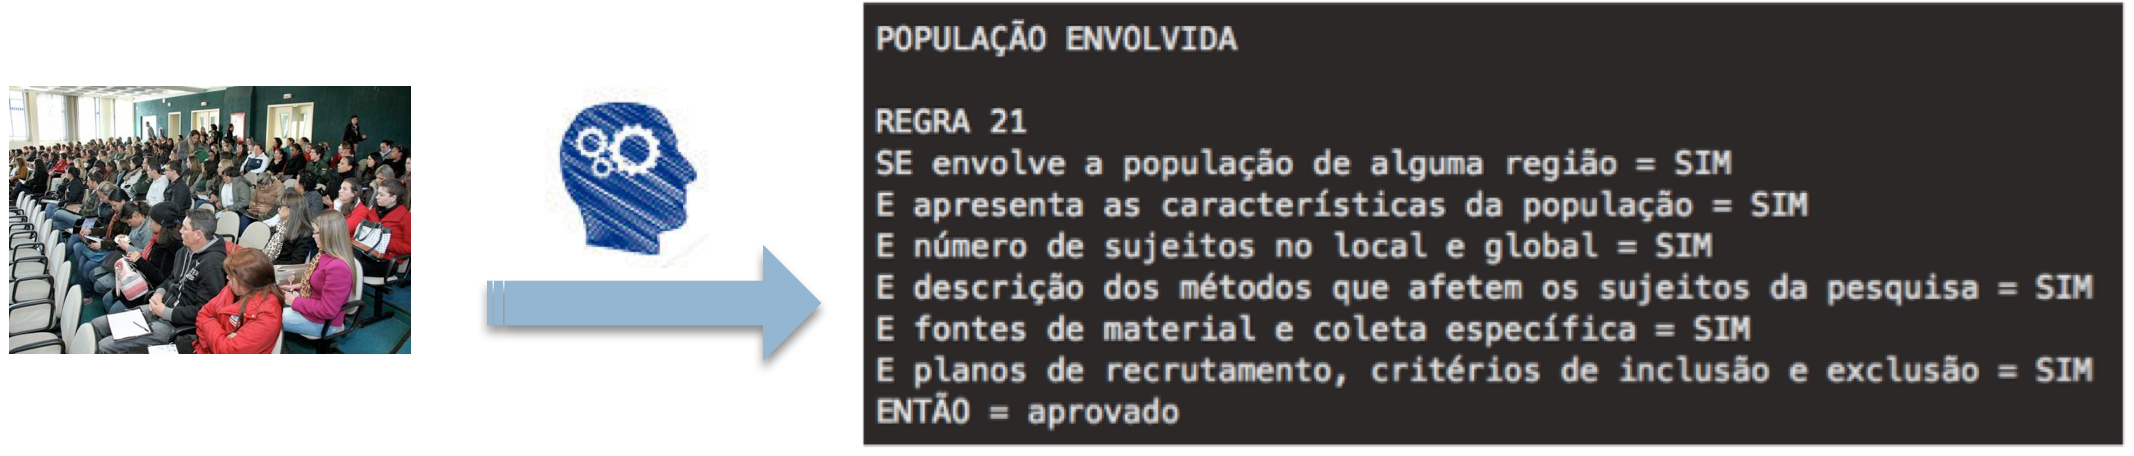
\includegraphics[width=\linewidth]{intro.png}
\end{figure}
\end{block}

\begin{block}{SiRP}
\textbf{Através de perguntas-chave com feedback é possível guiar o pesquisador novato durante as seções e alíneas das resoluções 466/12 e 510/16 de maneira a ensiná-lo a pré-avaliar seus próprios projetos que serão submetidos a Plataforma Brasil.}

\begin{figure}
\vspace*{1cm}
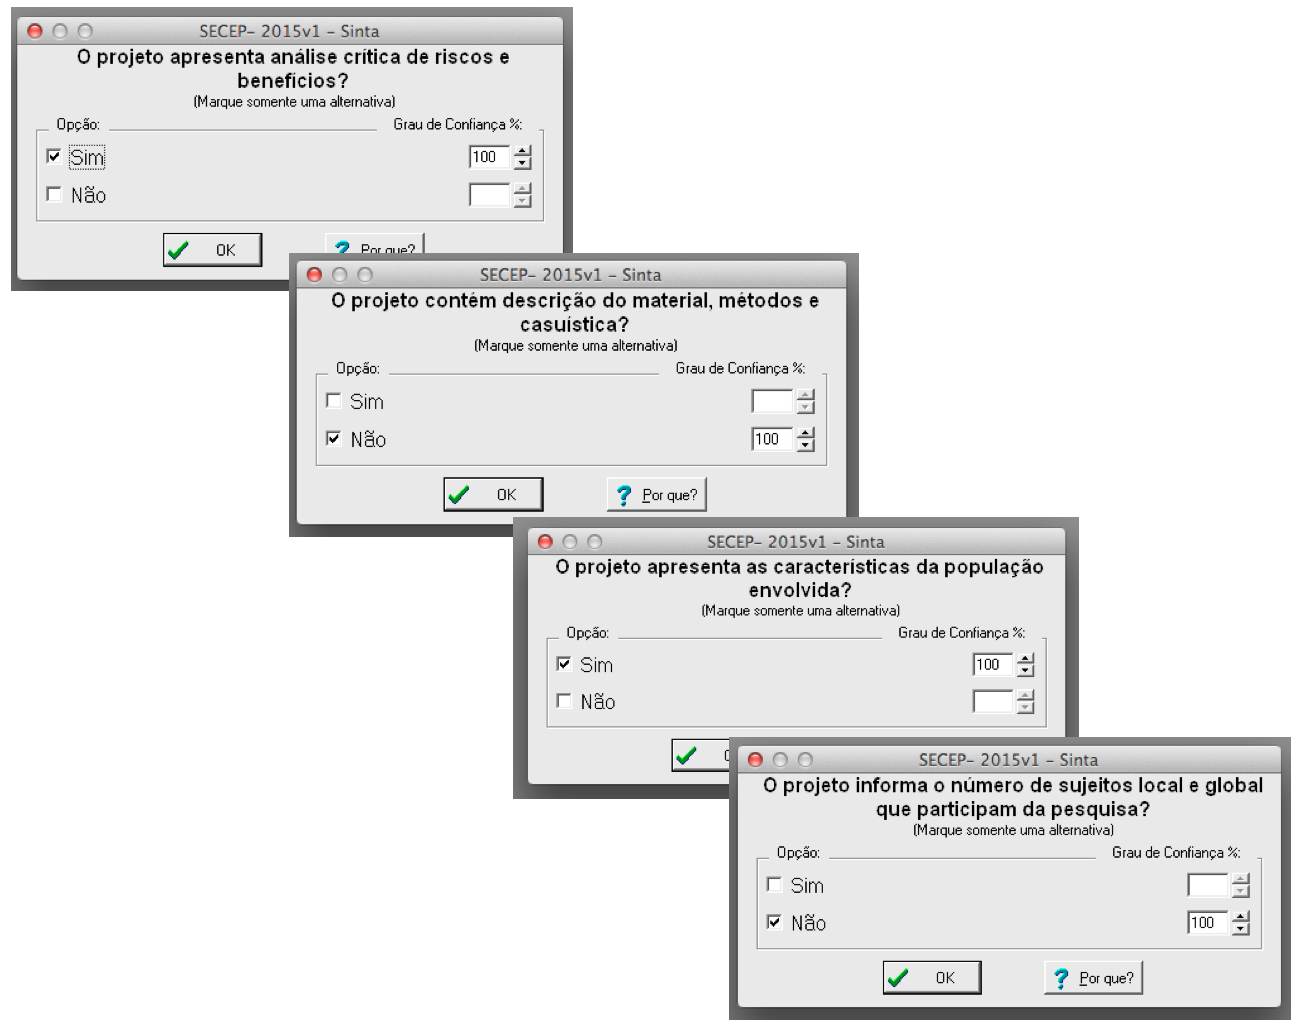
\includegraphics[width=.85\linewidth]{telas.png}
\end{figure}
\end{block}

\begin{block}{Como SiRP auxilia?}
\textbf{Perguntas são enviadas ao pesquisador, simulando uma conversa entre Relatores e Pesquisador, para pré-diagnosticar sobre cada um dos elementos descritos no protocolo de pesquisa.}
\end{block}

\end{column} %fim coluna 1
\begin{column}{\sepwid}\end{column} % separador coluna
\begin{column}{\onecolwid} %The second column
\vspace{1em}
 \begin{block}{Implementação com Inteligência Computacional}
 \textbf{SiRP contém uma base composta por 25 regras de conhecimento, embarcando um vasto estudo de 247 relatorias. Seguindo as orientações da literatura da Engenharia de Software, a base de conhecimentos, que está na sua segunda versão, foi redesenhada do antigo projeto SECEP. A escolha deste modelo se fez pelo fato de combinar a expansibilidade e a tolerância a mudanças.}

 \begin{figure}
 \vspace*{1cm}
 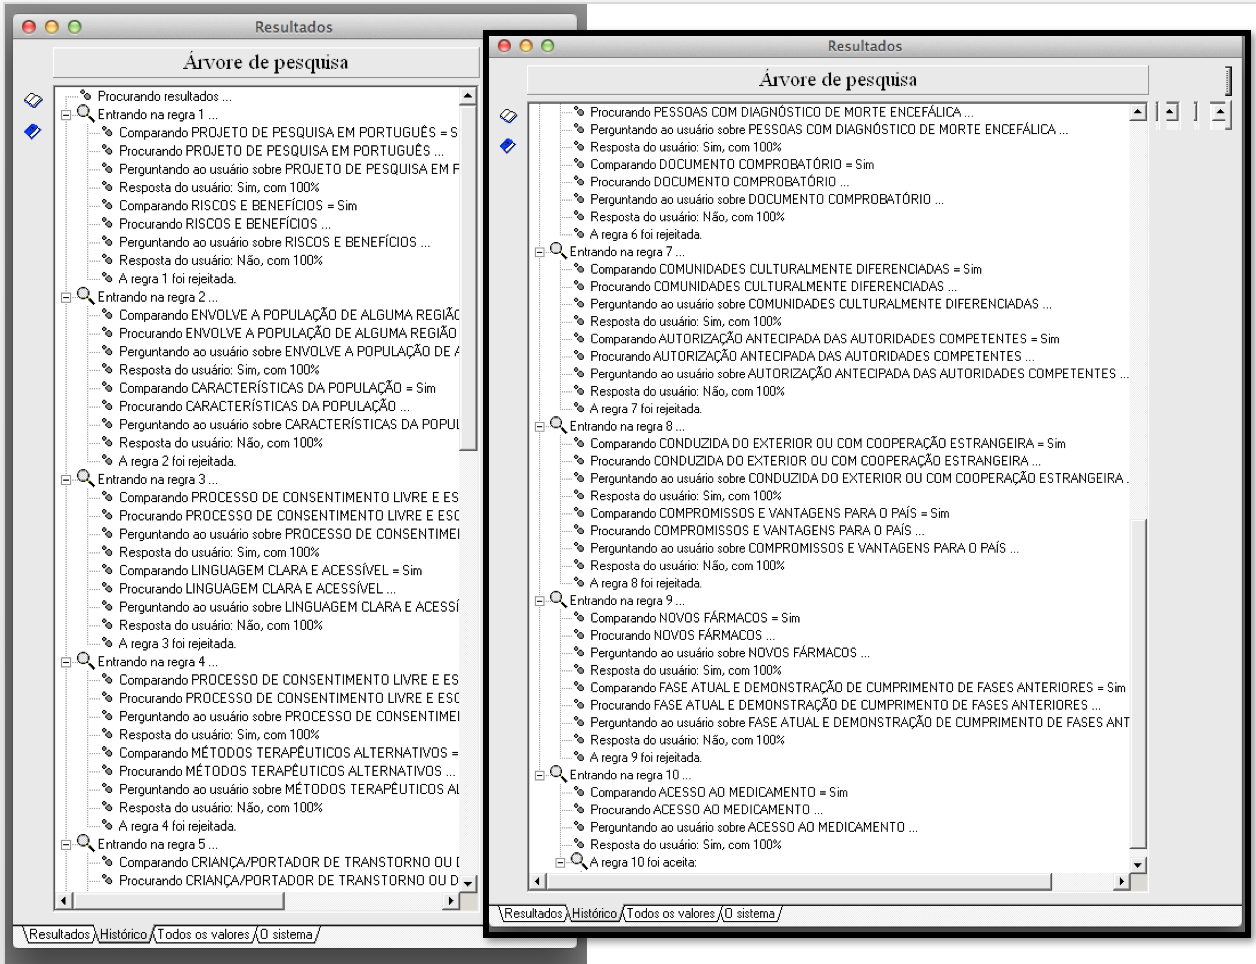
\includegraphics[width=.85\linewidth]{regras.png}
 \end{figure}
 \end{block}

      \begin{block}{Resultados}
 \textbf{Resultados preliminares durante a elaboração de projetos de pesquisa, enquanto se implementava o SiRP no laboratório de desenvolvimento de software, indicaram ganho de tempo na checagem do projeto, obtendo-se entre 43-75\% falhas em projetos-teste que não seriam detectadas por pesquisadores novatos - haja visto que em condições normais, o pesquisador novato necessitaria de mais tempo e treinamento.}
 \end{block}

 \begin{block}{Considerações Finais}
 \textbf{SiRP já pode ser utilizado fora do laboratório para prestar suporte imediato em suas tomadas de decisão sobre as resoluções, além de prestar suporte imediato para os treinamentos e minicursos durante a utilização dos conhecimentos na realização de projetos de pesquisa.}
 \end{block}

 \begin{block}{Agradecimentos}
 \begin{figure}
 \vspace*{.4cm}
 
\includegraphics[width=\linewidth, height=15cm]{agrdeco.png}
 \end{figure}
 \end{block}


\end{column}%fim coluna 2
\begin{column}{\sepmargin} \end{column}
\end{columns}
\end{frame}

\end{document}
